\chapter{Estado del Arte}

Con el desarrollo de la las tecnologías de secuenciación masiva los biólogos moleculares se han visto en la necesidad  de utilizar metodologías computacionales para analizar datos biológicos a gran escala, además de la aplicación de estas tecnologías en medicina requieren de un diseño y una validación que permita obtener nuevos conocimientos que sean  aplicables en la salud de los colombianos.

Este capítulo presenta el estado del arte de la secuenciación y de propuestas para análisis de datos biológicos. Esta organizado en biología molecular y secuenciación masiva, bioinformática y  minería de datos genómicos.  

\section{Biología molecular y secuenciación masiva}

Desde  que  Watson y Crick propusieron la estructura del ADN en 1953 \cite{Watson1953}, el estudio del ADN ha sido básico en el desarrollo de la biología molecular, incluso el mismo Francis Crick fue quien propuso el dogma central de la misma para describir la relevancia del ADN en los seres vivos y la utilización de la información que contiene por las células. Dada la importancia del  ADN  en las décadas de 1970 y 1980 se desarrollaron  técnicas para determinar el orden de los nucleótidos  (técnicas de secuenciación) de manera más eficiente que la secuenciación de las proteínas, y se definieron secuencias de algunos organismos como el virus de Episten Barr y  de la mitocondria humana, mediante la utilización de métodos químicos propuestos por Maxam y Gilbert en 1977 y Sanger en 1980 siendo este último el más popular; estas técnicas son conocidas como técnicas primera generación \cite{Herraez2012}. \\

Los métodos desarrollados para secuenciar prosperaron y con el proyecto del genoma humano, que comenzó en 1980 y fue completado en el 2003, permitieron que se desarrollaran nuevas tecnologías para optimizar el proceso de secuenciación y disminuir sus costos. Inicialmente, fue el secuenciador de Illumina  que en el 2008 permitió obtener el primer individuo humano secuenciado con esta tecnología \cite{Pei}. Estas nuevas tecnologías se fueron desarrollando en otras plataformas, tales como el secuenciador de roche 454 y el SOLiD de applied biosisten \cite{Pei} y son conocidas como tecnologías de última generación o de siguiente generación (Next-generation sequencing, NGS), que tienen la capacidad de realizar secuenciaciones de alto rendimiento de una maneras más rápida y económica que las de primera generación \cite{Herraez2012}. La diferencia entre las técnicas de secuenciación de primera generación y las de NGS se presenta en el hecho de que la nueva generación genera lecturas de menos de 500 pares de bases en comparación a las 1000 pares de bases de sanger \cite{Pei,Kulski2016}. \\
 
El desarrollo de estas tecnologías ha hecho que los datos genómicos aumenten de una manera vertiginosa, y permiten que se pueda realizar análisis en diferentes organismos con aplicaciones en biotecnología y salud \cite{Herraez2012}. Se ha estimado que cada genoma humano tiene alrededor de 3.5 millones de diferencias con respeto al genoma de referencia (Genoma de consenso para la salud humana), estas diferencias son llamadas variantes y pueden determinan el fenotipo de los individuos, algunas de estas variantes son conocidas para indicar predisposiciones a enfermedades \cite{Kutzera2017}.\\

En el campo de la salud actualmente se emplea la secuenciación de exomas, es la más utilizada puesto que se considera que los exones son las regiones de ADN conservadas y expresadas, (se traducirán en ARNm y posteriormente en proteínas) y representan menos del 2\% el genoma humano, pero se estima que contiene el 85\% de las variantes conocidas de enfermedades, lo que permite la reducción de costos y una buena alternativa frente a la secuenciación de genomas completos \cite{Illumina2017,Klug2013,Herraez2012}.\\

Dado que la utilización de NGS permitió entender enfermedades raras, fue posible identificar las regiones responsables de una enfermedad, teniendo como control los datos poblacionales a partir de proyectos de secuenciación como el proyecto de 1000 genomas. Los datos genómicos también pueden ser útiles para la caracterización de enfermedades poligénicas y su asociación con las variaciones genómicas presentes en el individuo \cite{Poliakov2015}. 

\subsection{Identificación de variantes}

La secuenciación de exones (secuenciación de exoma) ha sido un buen método para: \textit{i)} identificar SNPs (Polimorfismos de Nucleótido Único) y las SNV (Variantes de nucleótido simple) como se observa en la figura \ref{fig:snp}, \textit{ii)} identificar pequeñas delecciones o inserciones (indels) que pueden  ser  causales de enfermedades, y \textit{iii)} para explicar la variación fenotípica de los individuos \cite{Deng2011,Wenger2017}.\\

\begin{figure}[h!] 
	\centering
	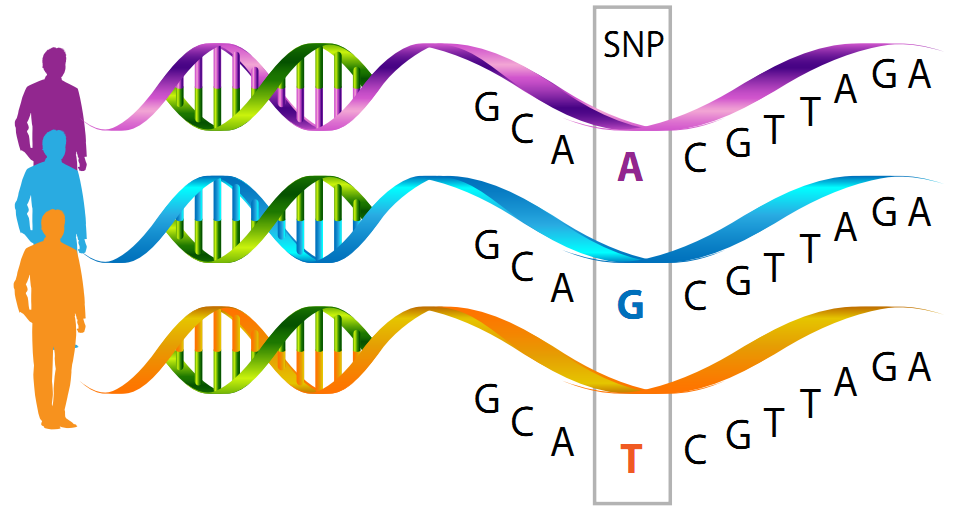
\includegraphics[width=0.5\textwidth]{Estado/snp}
	\caption{SNPs en Humanos.} \label{fig:snp}
\end{figure}

Las variantes de nucleótido simple (SNV) se clasifican según el cambio que generen a nivel de proteína en: \textit{variantes sinónimas}, que son aquellas donde el cambio de un nucleótido no genera cambios en la proteína, las \textit{variantes no sinónimas} que son las que generan un cambio en uno o varios aminoácidos de la proteína, \textit{variantes stopgain} y \textit{stoploss} que son variantes que generan una proteína más corta o larga de lo normal, \textit{variantes frameshift} que son \textit{delecciones o inserciones} que alteran el marco de lectura y finalmente \textit{variantes no frameshift} correspondientes a las \textit{delecciones y/o inserciones} que no alteran el marco de lectura \cite{Liu2016}.\\


A partir de la información pública disponible se ha estimado que las variantes pueden afectar la función de la proteína y al mismo tiempo pueden estar asociados a otros genes dentro de una enfermedad. En genética humana cuando una variante se presenta en una alta frecuencia dentro de la población es clasificada como benigna (no causa una enfermedad) pero en asociación con otra variante la convierte en causal de enfermedad, por ello la importancia de la integración de la información y la revisión de la variante \cite{Shendure2016}.\\

La identificación de variantes se realiza con diversas plataformas siendo el MiSeq un sistema de secuenciación de illumina  más popular a nivel mundial dado su relación costo-efectivo para la identificación de variantes, esta plataforma permite la secuenciación de 4813 genes en un solo experimento \cite{Illumina2017}. En cuanto al análisis de los datos esta plataforma incluye un servicio de computación en la nube (\textit{BaseSpace}), donde los datos biológicos son analizados  sin necesidad de que los investigadores tengan habilidades en bioinformática pero están disponibles como herramientas solamente de investigación y no como diagnóstico. A pesar de ser herramientas de investigación  que han sido desarrolladas, Illumina permite que dentro del BaseSpace se publiquen nuevos algoritmos, herramientas abiertas o aplicaciones diseñadas por desarrolladores con el objetivo de mejorar estos análisis genómicos y  de poder implementarlos en las diversas plataformas de secuenciación que ofrece esta la empresa Illumina \cite{Illumina2017}. \\

Los datos obtenidos a partir de técnicas de NGS han tenido un crecimiento vertiginoso y presentan un reto para el manejo y análisis de los mismos, debido a que los formatos de los datos y las inconsistencias de las secuencias como resultado de los procesos experimentales, la importación de las secuencias a nivel digital, el ensamble de los fragmentos de ADN, el alineamiento y post-alineamiento de grandes cantidades de datos biológicos hace que se convierta en una de las bases de la investigación en bioinformática \cite{Deng2011,Triplet2014}.

\subsection{Secuenciación de siguiente generación (NGS) aplicada en salud}

La secuenciación de siguiente generación(NGS) ha sido adoptada en el ambito clínico, dado que se ha documentado su utilidad para el diagnóstico de enfermedades  y para la toma de decisiones en cáncer o para la selección de dosis de medicamentos en un paciente, \cite{Lubin2017} algunos de estos ejemplos son:

\subsubsection*{Cáncer de Seno}

El cáncer de seno es una enfermedad que afecta principalmente a mujeres y que en estadios avanzados tienen una alta tasa de mortalidad por lo que ha recibido una importante atención de por la comunidad de investigadores, principalmente en el área biomédica con la intención de buscar marcadores genéticos de la enfermedad. Actualmente se encuentra una gran cantidad de investigaciones publicadas, donde se intenta visualizar las interacciones de los genes como esos marcadores en las distintas poblaciones \cite{Jurca2016}.\\

Teniendo en cuenta que el cáncer el resultado de una mutación de ADN, donde la consecuencia es que la célula portadora de la mutación pierda su funcion normal y gane la habilidad de multiplicarse de manera indefinida sobre los tejidos normales. Donde la identificación más común para realizar la identificación de biomarcadores geneticos es la utilización de NGS, donde la variación de un gen puede alterar la función celular y se causal de la enfermedad y en algunos casos puede ser heredable y predisponente al desarrollo de la enfermedad \cite{Jurca2016,Wenger2017}.


\subsubsection*{Fibrosis Quistica}

La fibrosis quística es una enfermedad multisistemica causada por mutaciones puntuales en el gen CFTR, las características típicas de esta enfermedad son: la enfermedad pulmonar obstructiva, infecciones bacterianas crónicas de las vías respiratorias y senos paranasales e infertilidad masculina debida  a azoospermia obstructiva, la mayoría de los pacientes con esta enfermedad tienen insuficiencia pancreática, es frecuente que los pacientes con fibrosis quistica tengan mutaciones en el gen CFTR con un efecto funcional de la proteína leve, se han identificado 2000 variantes asociados a esta enfermedad \cite{Terlizzi2017}. 


\section{Bioinformática}


La bioinformática según la asociación americana de patología y el colegio americano de patología es la disciplina que conceptualiza la biología en términos de macro-moléculas y aplica técnicas informáticas (matemática aplicada, ciencias de la computación y estadística) para entender y organizar la información asociada a esas macro-moléculas, en gran escala \cite{Roy2018}.\\  
 
La bioinformática combina retos de investigación en las áreas de la biología y la informática para desarrollar diferentes métodos y herramientas para el análisis de datos biológicos y puede tratar acerca  del almacenamiento, simulación y análisis de datos biológicos aplicando el uso de herramientas computacionales  como la minería de datos, esta ultima siendo definida como una herramienta de investigación, desarrollo y aplicación para expandir el uso de los datos biológicos y médicos con fines de investigación y generación de nuevos conocimientos, incluyendo las herramientas que permitan almacenar, archivar y analizar o visualizar dichos datos \cite{Littlefield} \\

El auge de las tecnología de NGS permitió que la bioinformática diera respuesta a las dificultades que presenta la genómica en la búsqueda de ser una nueva innovación biomédica y en otras áreas de las ciencias biológicas, donde el valor de la bioinformática radica en la promesa de que la información genómica tiene grandes beneficios que son aplicables al área de la salud aunque estos la obtención de información relevante presentan un varios retos uno de ellos es la integración de los datos genómicos y clínicos y los derechos de propiedad sobre los mismos\cite{Searls2010}. 

\subsection{Integración de datos genómicos y clínicos}

En la era de las omícas, los datos se presentan en diferentes formas y en varios niveles en términos biológicos, los cuales incluyen los datos genómicos, datos de transcriptomica, epigenomica, metabulomica, entre otros, donde se incluyen también las diferentes datos poblacionales humanos y las historias clínicas, la escala de estos datos se encuentran  entre  pentabyte y exabyte \cite{Li2014}.\\

Aunque la definición de “big data” es muy discutida dentro de las ciencias de la información, sin embargo el nombre se hace referencia a la “gran cantidad de datos” que se caracterizan por el volumen del procesamiento, la variabilidad de los mismos y la veracidad de la calidad de los datos \cite{Li2014}. Partiendo de lo anterior los datos genómicos  pueden ser catalogados como “big data” ya que poseen las siguientes características: Son numerosos, no pueden ser almacenados dentro de una base regular de datos, la velocidad  de generación y procesamiento es muy rápida \cite{Hashem2015}. \\

En el diagnóstico de enfermedades los datos genómicos vistos como "big data" comparten los mismos retos tecnológicos como son: el almacenamiento, la transferencia de la información, control del acceso y manejo de la información, otros retos computacionales propios de los datos es el moldeamiento de los sistemas biológicos, la gran escala y diversidad de los datos donde los modelos no optimizados que pueden fallar \cite{Ren2015}. \\

Las nuevas tecnologías de análisis genético son fáciles y económicas de hacer lo que genera una gran cantidad de datos biológicos y lo que hace que los biólogos trabajen cada vez más con las nuevas tecnologías de análisis genético, haciendo que los biólogos trabajen más y más computacionalmente. Especialmente mediante el uso de  tecnologías de secuenciación (NGS) y presentar un reto para integrar y almacenar la información, pasos que son necesarios para su posterior análisis \cite{Li2014,Cook2016}.\\

La gran cantidad de datos presentan un reto para organizar y manejar datos que crecen de manera exponencial y que son de diversos tipos, dado que los datos son generados a diferentes niveles y con diferentes métodos (ejemplo: Variantes de exones o imágenes de patología), datos que a su vez deben ser almacenados en distintas formas, esta situación muestra una seria dificultad para realizar un análisis integral de los datos \cite{Cook2016,Li2014}.\\

El problema de la heterogeneidad  de los datos  se aplica igualmente a los datos clínicos que describen pacientes individuales y además a los datos biológicos que caracterizan nuestro genoma. Específicamente la información genómica y clínica son datos altamente heterogéneos con respecto a los modelos de datos que emplean normalmente, los esquemas de datos que especifican, los lenguajes de consulta que soportan y las terminologías que reconocen \cite{Sujansky2001}.\\

Para el caso de las secuencias de genomas se tiene que para cada individuo tiene 3.2 millones de bases, que al ser comparadas contra un genoma de referencia muestran los cambias que cada individuo posee, estas variantes son almacenadas normalmente en el formato VCF (Formato de llamado de variantes), a su vez estos archivos pueden contener varias gigas de información, que representan un problema para el almacenamiento dentro de las bases de datos,y por lo tanto se hace necesario que se desarrollen soluciones dependientes de las diferentes características y necesidades de los laboratorios\cite{Kutzera2017}.\\

Para el manejo de los datos se han aplicado varios modelos de sistemas de información en  bioinformática con diversas herramientas para integrar datos biológicos, utilizando por ejemplo sistemas de bodega de datos; que están disponibles de manera gratuita y que fueron desarrollados con el fin de dar respuesta algunos de los problemas en el manejo de datos biológicos, dada la importancia que tiene de poder utilizar toda la información necesaria de manera eficiente se han propuesto diversas soluciones \cite{Triplet2014}, algunas de estas bases de datos públicas son las de NCBI y ensambl  que hacen parte de un consorcio internacional \cite{Sherry2001,Yates2016}.\\

Muchas  herramientas han sido implementadas con fines de investigación, más no con fines diagnósticos,  en este sentido se han implementado otras herramientas que permiten integrar datos con fines diagnósticos, ya que en este caso se requieren parámetros de seguridad por los datos que contienen información clínica y que deben ser manejados de manera privada. Esto implica otro manejo de datos biológicos ya que se adicionan nuevos datos como condiciones del paciente, tratamientos entre otros datos \cite{Canuel2015}. El cuadro \ref{tabla} presenta algunos de los software para integrar datos con fines de diagnósticos.\\

\begin{table}[h!]
	\centering
	\begin{tabular}{|p{5cm}|p{10cm}|}
		\hline
		Software     & Descripción                                                                                                                                                                                                                                                                                                                                                                                 \\ \hline
		BRISK: Biology-Related Information Storage kit      & Es un paquete de recursos abiertos, permite relacionar una descripción fenotípica y una mutación somática (SNP), lo que permite a los investigadores proveer una asociación de estudios genómicos y capacidades de análisis, teniendo en cuenta el manejo de la muestra \cite{Triplet2014}.     \\ \cline{1-2}
		CaTRip       & Fue desarrollada como un componente de caBIG, este software permite encontrar pacientes con perfiles similares, teniendo en cuenta el registro que hay dentro del sistema de datos clínicos, permite almacenar, cualificar y analizar datos de diferentes tipos de cáncer \cite{Canuel2015}.       \\ \cline{1-2}
		CBio Cancer Genomics Portal & Es otra herramienta que permite integrar datos definidos en la historia clínica de un paciente, como su descripción fenotípica, con la mayor cantidad de datos de ADN, ARNm, proteínas y de las imágenes obtenidas dentro de los diferentes exámenes realizados al paciente  \cite{Canuel2015}.                                                                                                                                                                                                              \\ \hline
		G-DOC Georgetown Database of Cancer & Fue desarrollada para integrar datos de las características de los pacientes con los datos biológicos, esta herramienta se enfoca en la visualización y análisis de datos \cite{Canuel2015}.                                                                                                  \\ \cline{1-2}
		iCOD Integrated Clinical Omics Database     & Esta herramienta combina la patología clínica de los pacientes y la información molecular de pacientes con el fin de dar una información holística de los pacientes, fue desarrollado de manera local y permite la visualización de mapas de enfermedades que permite la interrelación clínica con los datos biológicos \cite{Canuel2015}.      \\ \hline
		
		iDASH Integrating data for analysis, anonymization and sharing & No es una herramienta, pero si es un a infraestructura poderosa que permite la integración de datos y su análisis, distribuye herramientas y algoritmos enfocados en la privacidad de los datos \cite{Canuel2015}. \\ \cline{1-2}
		
		tranSMART & Es una herramienta abierta que permite a los investigadores hacer relaciones entre el fenotipo y los datos moleculares, Da a los investigadores herramientas para generar descripciones y análisis estadísticos \cite{Canuel2015}. \\ \hline 
	\end{tabular}
			\caption{Software de integración de datos genómicos con fines diagnósticos}	
			\label{tabla}
\end{table}

Otras herramientas han sido desarrolladas para encontrar asociaciones de variantes y genes afectados con las enfermedades requieren que se combinen los análisis de variantes con los individuos donde se tenga acceso a la información de manera eficiente \cite{Kutzera2017}. Algunas implementaciones desarrolladas para hacer esta tarea se presentan en el cuadro \ref{r1}.

\begin{table}[]
	\centering
	\begin{tabular}{|p{5cm}|p{10cm}|}
		\hline
		Software     & Descripción                                                                                                                                                                                                                                                                                                                                                                     \\ \hline
		Variant-DataBase (Variant-DB) within      & Es una base de datos implementada en PostgreSQL junto con Django para almacenar y manejar datos genómicos que se con tranSMART para asociar las variantes a un fenotipo \cite{Kutzera2017}.      \\ \cline{1-2}
		HGVD       & Es una herramienta con acceso web que permite manejar las variantes dentro de la población japonesa obtenidas a partir de secuenciación de exomas y genomas implementada en en PostgreSQL y la interfaz grafica con JBrowse \cite{Higasa2016}.       \\ \cline{1-2}
		Variome Project    &   Es un proyecto no gubernamental internacional que trabaja para integrar las variaciones genéticas y su efecto en la salud humana y que a su vez esta información sea curada, interpretada y compartida de manera gratuita \cite{variome2017}.                                                                                                                                                                                                              \\ \hline
	\end{tabular}
        \caption{Software de integración de variantes con enfermedades}
		\label{r1}
\end{table}

\subsection{Análisis de datos genómicos con aplicaciones clínicas}

A nivel mundial se han clasificado los datos genómicos en cinco tipos que son de gran tamaño y que son ampliamente usados en la investigación en bioinformática, estos datos son: 1) Los datos de expresión génica, 2) datos de secuenciación de ADN, ARN y proteínas, 3) los datos de interacciones entre proteínas (PPI), 4) datos de rutas metabólicas y 5) los datos de gene ontology (GO). Además se encuentran los datos de redes donde se asocian los genes con enfermedades que tienen una alta importancia en la investigación y el diagnóstico \cite{Kashyap2015}.\\

Dentro del análisis de datos de secuenciación los desarrollos se han enfocado en el manejo de la gran cantidad de información generada, mientras que en las asociaciones con enfermedad se enfocan en la asociación multi-objetivo entre la enfermedad  y las redes heterogéneas son utilizados para establecer la relaciones entre los genes y la enfermedad; la complejidad de estas relaciones implican la utilización de herramientas de aprendizaje de máquina para reorganizar y visualizar la gran cantidad de datos obtenidos, y así poder realizar análisis y diagnóstico de enfermedades \cite{Kashyap2015}. \\

Dentro de las secuencias para el análisis a gran escala se ha utilizado la plataforma de Hadoop MapReduce, utilizando también BioPig  como herramienta que se basa en el análisis de secuencias a nivel masivo utilizando la arquitectura de MapReduce, otra herramienta está el Crossbow que se combina con Bowtie para dar una respuesta ultrarrápida con un uso eficiente de memoria para el alineamiento de lecturas cortas y SoapSNP que permite la identificación de SNP en genomas completos a través de computación en la nube o de manera local utilizando un clúster de hadoop. Otras herramientas basadas en la nube son Stormbow, CloVR y Rainbow. Otras plataformas que no utilizan herramientas de big data son Vmatch y SeqMonk \cite{Kashyap2015}.\\

Una de las herramientas más populares para el manejo el análisis de secuenciación de alto son Galaxy Project que permite el análisis de los diferentes tipos de datos por medio de una interfaz web o de manera local y es un software libre, también permite crear flujos de trabajo automatizados [17]. Otra herramienta es GATK que fue desarrollada por el Broad Institute y que se enfoca en el descubrimiento de variantes  a diferentes niveles y con diversos organismos y con usos investigativos [18]. GATK a diferencia de Galaxy Project no tiene una interfaz gráfica y debe ser instalado en equipos con Linux y basa su arquitectura utilizando hadoop MapReduce para el procesamiento de los datos \cite{Maharjan2011} .\\

Igualmente se han realizado implementaciones para análisis  en bioinformática implementado los algoritmos de alineamiento múltiple en Hadoop  y utilizando HBase, paralelizando la versión del NCBI del algoritmo BLAST, también se ha aplicado a nivel clínico la cantidad de datos producidos por los laboratorios como los record médicos electrónicos, datos biomédicos, datos biométricos, expresión génica entro otros y  se ha utilizado el framework de MapReduce para realizar análisis simultáneo con un retorno rápido de resultados, haciendo que la promesa de que los análisis de “big data”  en bioinformática y la salud sea aplicable \cite{Mohammed2014}.\\

Cada una de las herramientas han sido desarrolladas para responder al manejo datos en bioinformática y su análisis,  Colombia se ha propuesto el usos de las bodegas de datos para dar soporte a la investigación, ya que el uso de estas metodologías han sido ampliamente aplicados en inteligencia de negocios, y se presenta la modelación multidimensional de datos biomédicos basados en bodega de datos \cite{Bustos2007}.\\

Bustos \cite{Bustos2007}  y colaboradores proponen que la bodega de datos aplicable en bioinformática es  un hibrido entre Data Warehouse (bodega de datos) y data marts, utilizando la aplicación de descubrimiento de conocimiento (KDD) en los datos almacenados. El modelo propuesto es: 1) Selección de datos. 2)  agrupamiento y 3) clasificación. En bioinformática se han aplicado las técnicas de minería para tratar de resolver diversos problemas biológicos, dependiendo del tipo de problema que se quiera abordar. Por ejemplo para la exploración de variantes de nucleótido simple (SNPs) asociados a enfermedades se ha implementado el algoritmo Apriori para buscar dentro de un set de atributos reglas que sean consistentes con la literatura, teniendo en cuenta que existen millones de SNPs que están correlacionados con varios fenotipos \cite{Staccini2014}.

\section{Minería de datos genómicos}

La minería de datos (visto desde la bioinformática) es  el proceso de extraer nuevo conocimiento (previamente desconocido) de datos biológicos, esto permite también la utilización de conceptos de minería de datos y aprendizaje de máquina  con aplicaciones en la investigación biológica, dependiendo de los datos que se estén utilizando para ser aplicados, se encuentran los genómicos que provienen del secuenciación de ADN, los transcriptomicos que son de secuenciación de RNA o los de proteínas que provienen de las inferencias y los datos experimentales desde la química \cite{Farid2016}. \\ 

Las inferencias con respecto a las grandes cantidades de datos genómicos requieren análisis computacionales para interpretar los datos, siendo una de las áreas más activas en la bioinformática, donde se utiliza la minería de datos (entiendo la minería de datos como el método de extraer información por medio del aprendizaje de máquina, la estadística, la inteligencia artificial, patrones de reconocimiento y visualización) para resolver problemas biológicos, algunos ejemplos donde se ha aplica técnicas de minería es la clasificación de genes, análisis de mutaciones en cáncer y en la expresión de genes \cite{Littlefield}. \\

También han sido aplicadas técnicas de agrupación de genes expresados diferencialmente, las máquinas de soporte vectorial han sido utilizados para asociar interacciones entre genes y generar redes biológicas, igualmente las metodologías tradicionales de minería de datos en ocasiones no son precisas o eficientes y requieren que se desarrollen nuevos algoritmos y metodologías que respondan de una manera más acertada a una pregunta biológica \cite{Zaki2007}. Sin olvidar que se requiere evaluar las plataformas disponibles, las herramientas tecnológicas que permitan  la implementación de procesos que asocien los datos a  la investigación  y obtener resultados más generalizados.  Esto debe estar aplicado a los requerimientos de los investigadores para garantizar una implementación exitosa \cite{Bustos2007,Zaki2007}.\\

Algunas de las tareas de minería de datos son \cite{Littlefield}:

\begin{enumerate}[1.]
	\item Clasificación: Donde se clasifican los datos a una clase predefinida.
	\item Asociación: Ver elementos que están asociados mediante reglas
	\item El \textit{clustering} o agrupamiento: Como la definición de una población de datos dentro de un subgrupo o grupo .
\end{enumerate}

La utilización de las técnicas de secuenciación de alto rendimiento junto  la aplicación de técnicas de minería de datos pueden aportar al diagnóstico de enfermedades complejas  como las fallas cardiacas y el cáncer que presentan diversas causas \cite{Hannah-Shmouni2015}, partiendo de lo anterior se hace necesario saber la relación entre las moléculas biológicas y las características de una enfermedad vistas desde la alteración de uno o varios genes y las posibles alteraciones que estos causan en una persona \cite{Li2014}.

\subsection{Minería de texto en el campo clínico}

En los procesos médicos, la relación entre los factores que pueden afectar la salud juega un papel importante. Una de las relaciones más comunes es la relación entre los genes y las enfermedades donde la secuenciación de exones tiene una alta aplicabilidad. Pero la identificación manual de este tipo de relaciones es compleja dada la cantidad de características que se pueden presentar como el diagnóstico propio de la enfermedad y/o la respuesta a los tratamientos \cite{Kawashima2017}.\\

Actualmente, mucha de la información clínica se encuentra contenida en textos libres de publicaciones científicas, historias clínicas o bases de datos especializadas como OMIN, por esta razón el procesamiento del lenguaje natural en los últimos años ha tenido un impacto en la investigación clínica, además no puede ser aplicado en políticas de salud pública o usarse con fines diagnósticos. \cite{Neveol2014}\\

La minería texto puede ser aplicada en la medicina, esto implica la utilización del procesamiento del lenguaje natural dentro del contexto clínico y que sea implementado en diferentes idiomas \cite{Neveol2014}, donde el agrupamiento ha sido considerado uno de los métodos más importantes, ya que se basa en aprendizaje de máquina no supervisado y que ha sido aplicado a diferentes problemas\cite{Kawashima2017}, teniendo en cuenta que uno de los objetivos del agrupamiento de datos, es la  identificación de grupos naturales en datos sin etiquetas. Las tareas de minería datos en textos clínicos son las clásicas que se utilizan en minería de datos, como el preprocesamiento, el agrupamiento y la clasificación, donde los documentos son la información clínica, ya sea de historias clínicas o literatura médica \cite{Jain2010,Renganathan2017}.


\subsubsection{Preprocesamiento}

El preprocesamiento de documentos generalmente presenta dos pasos que son la remoción de stop words y el stemming. Las stop words son palabras que tienen una alta frecuencia y  que detienen una oración, como por ejemplo de, y, más, por,como etc y que tienen una alta frecuencia en los documentos. El stemming  que permite realizar una representación de las palabras desde su raíz convirtiéndolas en un solo término, por ejemplo, analiza, analizo y análisis que serian representadas por el término análisis \cite{Renganathan2017}.\\

Una vez realizado el preprocesamiento se preparan los datos se calcula la matrix de frecuencia de términos $tf$ y la frecuencia invertida de documentos $idf$; que son utilizadas para calcular la matriz $tfidf$ como uno de los métodos más populares para ponderar los términos, debido a que disminuye el peso de la ocurrencia de términos en la colección de los documentos, haciendo que la comparación entre los mismos no sea afectada por palabras distintivas que tienen bajas frecuencias en la colección\cite{Renganathan2017,Allahyari2017}. \\

El cálculo de la frecuencia de términos $\mathit{tf}_{i,j}$ y posterior mente el cálculo de la matriz tf-idf, que se realiza a partir de frecuencia invertida con la ecuación: 
$${idf}_i = \log_2 \frac{|D|}{|\{d \mid t_i \in d\}|}$$
siendo $|D|$ lo que denota el número total de documentos y donde $|\{d\mid t_i \in d\}|$ en  que $t_1$ aparece, la matriz de tf-idf es calculada a partir de la multiplicación de la frecuencia de términos y la frecuencia invertida de documentos $\mathit{tf}_{i,j} \cdot \mathit{idf}_i$. Una vez obtenida la matriz $tfidf$ se normaliza y se utilizan los datos según las tareas de minería que se quieran aplicar, excepto para asociación que utiliza los datos presentes en el sistema de información. \cite{Buckley1988,VishalGupta2009}.

\subsubsection{Agrupamiento}

La tarea de agrupamiento es una de las más populares en minería de texto, tiene aplicaciones como la clasificación, visualización y organización de documentos. El agrupamiento encuentra grupos de documentos similares en la colección, donde la similaridad es computada mediante una función, y la granularidad de los documentos puede ser documentos, párrafos, oraciones o términos. Para desarrollar está tarea se pueden usar técnicas como el agrupamiento jerárquico o el agrupamiento particional \cite{Renganathan2017,Allahyari2017}.\\

\textit{Medidas de similaridad y distancias:} La eficiencia del proceso de agrupamiento depende las medidas de similaridad o distancia como son el coseno, la distancias euclidiana, la manhattan etc. Siendo la similitud de coseno la más utilizada, puesto que los términos son representados como vectores y la similaridad de dos documentos corresponde a la correlación entre esos vectores que es cuantificada como el angulo de esos vectores, además esta medida tiene como ventaja que es independiente del largo del ocumento \cite{Renganathan2017,Huang2008}.\\

Existen dos grupos en los que se puede dividir los algoritmos de agrupamiento y son en particionales y jerárquicos. Los algoritmos de agrupamiento jerárquico recursivamente encuentran grupos anidados en modo aglomerativo (comenzando con cada punto de datos en su propio grupo y fusionando el par más similar de grupos sucesivamente para formar una jerarquía de clúster) o en modo divisivo (de arriba hacia abajo) (comenzando por todos los puntos de datos en un gr upo y dividir recursivamente cada grupo en clústeres más pequeños).En la agrupación jerárquica, conocimiento previo sobre el número no se requieren grupos de grupos. El resultado de la agrupación es una representación gráfica llamada dendrograma,en el que los documentos están representados de forma jerárquica estructura de árbol que representa los documentos como sus ramas \cite{Renganathan2017,Jain2010}.\\

En comparación con los algoritmos de agrupación jerárquica, los algoritmos de agrupamiento  particional encuentran todos los grupos simultáneamente como una partición de los datos y no imponen una estructura jerárquica, siendo el k-means el algoritmo más popular \cite{Jain2010}. \\

El k-means inicia con un número predefinido de grupos de documentos, por cada instancia, $k$ grupos, al utilizarlo con los documentos estos se ubicaran en diferentes grupos según  la cercania del centroide del grupo (media). En cada iteración, el centroide del grupo se vuelve a calcular recursivamente después de la reubicación de los documentos en función de la proximidad al centroide del grupo. Esto se repite hasta que no haya cambios en la reubicación de los documentos \cite{Renganathan2017}. \\

Para la selección del número de $k$ existen varios metodologías como son: el método del codo, este es uno de los métodos más antiguos para determinar el número de grupos, se realizan varios experimentos iniciando por un $K$  y realizando un incremento de 1, para los cuáles se calcula el costo que conlleva cada una de las iteraciones; entre más se aumente el número de $K$ el costo disminuye y el número de $K$ alcanza una meseta, este valor es el que se desea obtener, visualmente se realiza la identificación mediente un gráfico de error cuadrático y número de grupos, la razón es que al continuar el aumento del número de $K$ los nuevos grupos son muy cercanos a otros \cite{Kodinariya2013}.\\ 

Otra forma de seleccionar el número de $K$ es con el coeficiente de Silhouette que es una evaluación de los grupos, donde los valores altos son relacionados a modelos que tienen grupos es bien definidos. El coefiente está definido por cada muestra y está compuesta por dos valores que son \cite{scikit-learn,Rousseeuw1987}:

\begin{itemize}
	\item \textbf{a:} La distancia media entre una muestra y todos los puntos de la misma clase.
	\item \textbf{b:} La distancia media entre una muestra y todos los otros puntos en el próximo grupo más cercano.
\end{itemize}

El coeficiente Silhouette $s$ para una sola muestra se da como:

$$s = \frac{b-a}{max(a,b)}$$

Para un set de datos el coeficiente Silhouette es el promedio del coeficiente por cada muestra \cite{scikit-learn,Rousseeuw1987}. \\

\textbf{Validación de los grupos:}

Para los grupos obtenidos se pueden calcular  medidas de validación que están dentro de la librería scikit-learn \cite{scikit-learn} son:

\begin{itemize}
	\item  \textit{Homogeneidad:} Definida como donde cada grupo contiene solo datos de una misma clase.
	\item \textit{Integridad:} Donde todos los miembros de una misma clase son asignados al mismo clúster.	
	\item \textit{V-measure:} Es la medida armónica ente la homogeneidad y la integridad \cite{Rosenberg2007}. 		
\end{itemize}

El cálculo de la homogeneidad y la integridad del grupo es calculada:
$$h=1- \frac{H(C|K)}{H(C)} $$

$$c=1- \frac{H(K|C)}{H(K)}$$

donde $H(C|K)$ es la entropía condicional de las clases en cada asignación de grupo y que son calculadas por:

$$H(C|K)= - \sum_{c=1}^{|C|} \sum_{k=1}^{|K|} \frac{n_c,_k}{n} . \log \frac{n_c,_k}{n_k}$$ 

y $H(C)$ es la entropia de clases y es calculada:
$$H(C)=  - \sum_{c=1}^{|C|} \frac{n_c}{n} . \log \frac{n_c}{n}$$ 
con $n$ que es el número total de muestras $n_c$ y $n_k$ son el número de muestras asignadas respectivamente a la clase $c$ y al grupo $k$, y finalmente $n_c,_k$ son el número de muestras de las clases $c$ asignadas al grupo $k$.\\

Finalmente el V-measure está definido de la siguiente manera \cite{Rosenberg2007}:

$$v= 2.\frac{h.c}{h+c}$$

Donde $h$ es la homogeneidad del grupo  y $c$ la integridad del grupo. 

\subsection{Reglas de asociación para el análisis de variantes}

Las reglas de asociación es un método popular y bien investigado para describir las relaciones entre variantes en grandes bases de datos \cite{Hahsler2005}. Las reglas de asociación (RA) muestran atributos con valores que ocurren frecuentemente en el set de datos, es posible obtener todas las posibles reglas de algunos atributos según la presencia de otros atributos \cite{Karabatak2009}.\\

Las reglas de asociación se basan en un set de items(elementos) $I = \{i_1,i_2,.....i_n \}$ que son un conjunto de $n$ atributos binarios. También se tiene que $D = \{t_1,t_2,..... t_m\}$ son el número de transacciones en la base de datos, cada transacción $D$ tiene una identificación única y contienen un subconjunto de elementos en $I$. Una regla se define como una implicación de la forma $X \Rightarrow Y$ donde $X,Y \subseteq I$ y $X \bigcap Y = \emptyset$. Los sets de elementos son llamados $antecedentes$ y $consecuentes$ \cite{Hahsler2005,Karabatak2009}.La selección de reglas interesantes se realiza calculando la confianza y el soporte que son definidos como:

\begin{itemize}
	\item Dados un set de datos $X \Rightarrow Y$, en una \textit{regla de asociación} tiene una confianza $c$ si $c$ de nuestra transacción que contiene $X$ pero que también contiene $Y$ \cite{Agrawal1994}.
	
	\item Dados un set de datos $X \Rightarrow Y$ tiene una \textit{regla de asociación} tiene un soporte $s$ si $s\%$ de las transacciones en nuestra base de datos de transacciones que contienen $X\cup Y$ \cite{Agrawal1994}. 
	
	\item Los algoritmos de asociación tratan de encontrar todas las reglas que tengan un mínimo de soporte y un mínimo de confianza\cite{Agrawal1994}. 
\end{itemize}

\subsection*{Trabajos previos}

Algunas de las publicaciones que se han realizado en donde se aplican modelos de minería de texto utilizando agrupamiento y/o reglas de asociación son:

\begin{itemize}
	\item ``
	Clustering Similar Clinical Documents in Electronic Health Records" de Tang, C. y colaboradores presentado en International Conference on Data Science en el 2018. Que realiza la identificación de documentos similares mediante la recolección de historias clínicas electrónicas y con la utilización del algoritmo K-Means. Trabajo en el que se presentan como resultados la identificación de notas clínicas similares con un rango de precisión entre 80\% y 89.5\% en 9 diferentes tipos de notas y con un total de 30 grupos.
	
	\item ``A system for exploring big data: An iterative k-means searchlight for outlier detection on open health data" de Rao, A. y colaboradores presentado en Proceedings of the International Joint Conference on Neural Networks en el 2018 donde utilizan información clínica para identificar diagnósticos diferenciales, utilizando agrupamiento para detectar enfermedades complejas y recurrentes durante un periodo de tiempo con el fin de generar mejores planes de atención a los pacientes .  
	
	\item ``Lung Cancer Concept Annotation from Spanish Clinical Narratives" de Koike, T. y colaboradores presentado en  Data Integration in the Life Sciences. DILS 2018. y muestra una aplicación de procesamiento de lenguaje natural aplicado en español y con historias clínicas de pacientes con cáncer de pulmón en historias clínicas en español en búsqueda de patrones del desarrollo de la enfermedad. En este trabajo encontraron el estado de mutación del tumor y estadio de cáncer de pulmón de los pacientes analizados. 
	
	\item ``Aiding Remote Diagnosis with Text Mining" de Karlsson,R. y colaboradores presentado en Artificial Intelligence Research Society Conference en el 2018. Es un trabajo que plantea la propuesta de realizar identificación de diagnósticos basado en los síntomas del paciente sin necesidad de que el médico este presente dentro de la consulta, para este trabajo también se utiliza el K-means.  Donde obtuvieron 5 grupos de pacientes con diagnósticos similares 
	
	\item ``Discovering blood donor arrival patterns using data mining: a method to investigate service quality at blood centers."  de Testik,M. públicado en 2012 en la revista  Journal of medical systems y colaboradores en el cual desarrollan un modelo de minería para la identificación de donantes de sangre utilizado agrupación y clasificación, como resultado obtuvieron grupos de pacientes donantes y predicciones a futuro de pacientes donantes, esto con el fin de apoyar la disponibilidad de tipos de sangre en los bancos de sangre. 
	
	\item ``Detecting significant genotype–phenotype association rules in bipolar disorder: market research meets complex genetics" de Breuer, R y colaboradores que se público  en International Journal of Bipolar Disorders en el 2018, donde realizan una asociación de variantes en pacientes con trastorno bipolar y que puedan ser causales de esta enfermedad. De este modelo obtuvieron nuevas variantes  candidatas como causales o factores de riesgo a trastorno bipolar.

\end{itemize}


\section*{Resumen}

Se presentó el estado del arte de la secuenciación de siguiente generación y el impacto que ha tenido en el diagnóstico, pronostico y seguimiento de enfermedades complejas y las posibilidades de analisis y aplicaciones que puede traer el uso de estas tecnologías. Además se presentaron metodologías para gestionar,analizar y obtener información relevante a partir de los datos genómicos incluyendo técnicas de minería de datos como el agrupamiento y las reglas de asociación. 
